% (approx. 500-800 words)

\section{Evaluation}
\label{sec:eval}
The purpose of this section is to explain and show the obtained results across different runs. In particular, it is worth mentioning that
lots of default valued hyper-parameters have been used such as:
\begin{itemize}
    \item \textit{batch size}, for both the training of the BiSTM (\Cref{subsec:subj}) and the final polarity evaluation procedure, of $128$
        samples. In the case of the binary classifier (~\cite{sequence}), a batch size of $64$ has been used;
    \item concerning the \textit{dataset split} dimensions:
        \begin{itemize}
            \item the subjectivity dataset into training set ($80\%$) and test set ($20\%$). The training set has been further splitted 
            considering a randomly sampled $10\%$ for evaluation pruposes;
            \item the IMDB dataset has been splitted following the built-in splitting format of the dataset itself ($25K$ samples for training
            and $25K$ sampels for evaluation)
        \end{itemize}
    \item during the training procedure an \textit{early stopper} has been used to implement an early stopping techinque. To do so, the 
        difference between the accuracy at the previous run and the current one is investiagate. If the latter is grater than $MIN\_DELTA=0.075$, 
        then the training procedure is interrupted and the last model saved;
    \item the BiLSTM model has been trained for $10$ \textit{epochs} and the binary classifier just for one (for time reasons);
    \item regarding the BiLSTM model, the multiple runs have been performed using a randomly selected seeds: $[91, 11, 57, 822, 19]$;
    \item for the AdamW and Adam optimiers, the learning rates used are $0.001$ and $0.0002$ respectively. 
\end{itemize}


\subsection{Evaluation metric}
\label{subsec:metric}
Across the different models, several evaluation metrics have been used. 
\subsubsection{Baseline}
Concerning the baseline, a simple \texttt{accuracy} metric has been used across a 10-fold cross validation procedure.
\subsubsection{Custom model}
As regards my proposed model, different evaluation metrics have been used for the different components:
\begin{itemize}
    \item for the BiLSTM model, as well as for the final evaluation on the polarity dataset, to detect subjectivity labels, a simple cumulative accuracy metric, defined as the sum of all the agreeements
    across all the batches over the number of samples in the training set, has been used;
    \item for the \textit{BertForSequenceClassification} instance an ensamble of metrics has been computed, exploiting the 
    \texttt{accuracy\_score} and \texttt{precision\_recall\_fscore\_support} methods provided by the \texttt{sklearn} python module. 
    In particular, the function used to compute these metrics can be analysed in \textbf{\Cref{alg:binaryclf}}
    \item as for the BiLSTM model, also for the final polarity classification step a cumulative accuracy has been used, where the agreeements
    between the predictions given by the pre-fine-tuned binary classifier and the ground truth are investigated and quantified.
\end{itemize}


\begin{algorithm}
    \SetAlgoLined
    \DontPrintSemicolon
    \KwIn{pred}    
    \KwOut{accuracy, f1, precision, recall}
    \CommentSty{\color{blue}}
    precision, recall, f1, \_  $\gets$ precision\_recall\_fscore\_support(labels, preds, average='binary')\;
    acc $\gets$ accuracy\_score(labels, preds)\;

    return\{\;
            \hspace{5mm}'accuracy': acc,\;
            \hspace{5mm}'f1': f1,\;
            \hspace{5mm}'precision': precision,\;
            \hspace{5mm}'recall': recall\;
        \}

\caption{Metric computation function for Trainer interface.}
\label{alg:binaryclf}

\end{algorithm}

Of course, the overall objective is to maximise the accuracy on both subjectivity and polarity datasets by minimizing the losses used during 
the training procedure as application of the maximisation of the posterior probabilities.

\subsection{Results}
\label{subsec:res}
In this particular section, the results obtained across different runs and experiments are analysised as much in detail as possible.\\
\begin{figure}
    \centering
    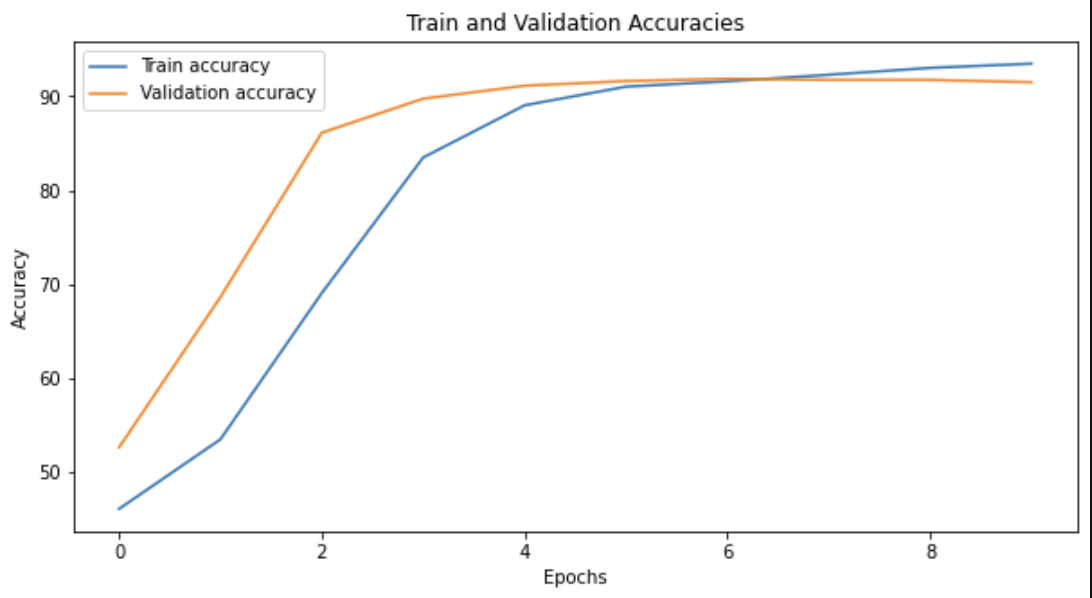
\includegraphics[scale=0.28]{Images/singlerunacc.png}
    \vspace{-1.0em}
    \caption{BiLSTM model training and evaluation accuracies on a single run.}
    \vspace{-1.0em}
    \label{fig:singlerunacc}
\end{figure}

\begin{figure}
    \centering
    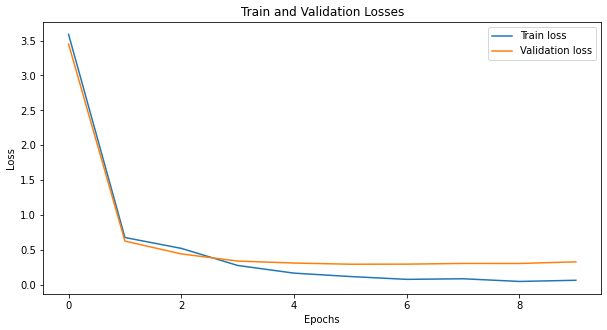
\includegraphics[scale=0.28]{Images/singlerunloss.png}
    \vspace{-1.0em}
    \caption{BiLSTM model training and evaluation losses on a single run.}
    \vspace{-1.0em}
    \label{fig:singlerunloss}
\end{figure}


In \textbf{\Cref{fig:singlerunacc}} and \textbf{\Cref{fig:singlerunloss}} it is possible to respectively appreciate the training and 
evaluation accuracies and losses, on a single run for the BiLSTM model (discussed in \Cref{subsec:cutsom}). \\
Since a single run is not very expressive and fully reliable, I decided to perform a 5-fold cross validation addressing both the average 
accuracy as well as the variance across the different runs (for details refer to \Cref{tab:crossval}).\\

\begin{center}
    \begin{threeparttable}
    \caption{5-fold cross validation subjectivity results using BiLSTM model}
        \begin{tabular}{cc}
            \toprule
            \thead{Seeds} & \thead{Accuracy} \\
            \hline
            $91$ & $89.5$ \\
            $11$ & $90.8$ \\
            $57$ & $91.05$\\
            $822$ & $90.25$\\
            $19$ & $89.1$ \\
            \hline
            Avg. Acc. & $90.14$ \\
            \hline
            Acc. Var. & $0.74$ \\
            \bottomrule
        \end{tabular}
        \label{tab:crossval}
    \end{threeparttable}
\end{center}

The main reason behind using a BiLSTM model is to try to better catch the dependencies between the words in a sentence. The results turned out to be worse than the ones obtained with the baseline from 
the cumulative accuracy perspective but better in terms of consistency and stableness. Indeed, using the same evaluation metric, the average statistics, listed in \Cref{tab:comparison}, 
shows that the baseline reaches a better percentual average accuracy but a higher variance across the different runs, i.e. seems to be more unstable and inconsistent.\\

\begin{center}
    \begin{threeparttable}
    \caption{Comparison between the baseline and the BiLSTM model}
        \begin{tabular}{ccc}
            \toprule
            \thead{Model} & \thead{Accuracy} & \thead{Variance}\\
            \hline
            Baseline & $90.75\%$ & $0.00013765$ \\
            Custom Model & $90.14\%$ & $5.534000000000004e-05$\\
            \bottomrule
        \end{tabular}
        \label{tab:comparison}
    \end{threeparttable}
\end{center}

Investigating the final results on the polarity dataset, it is possible to appreciate that the proposed model reaches a better accuracy than the baseline, as shown in \Cref{tab:finalres}.\\
It is worth mentioning that the "x" on the \texttt{accuracy} column of the table means that the model has not been tested multiple times on the polarity dataset since the latter is used just for evaluation
purposes as discussed in \Cref{subsec:mr}.\\

\begin{center}
    \begin{threeparttable}
    \caption{Comparison between the baseline and the proposed model}
        \begin{tabular}{ccc}
            \toprule
            \thead{Model} & \thead{Accuracy} & \thead{Variance}\\
            \hline
            Baseline & $83.2\%$ & $0.00112$\\
            Custom Model & $92.83\%$ & x\\
            \bottomrule
        \end{tabular}
        \label{tab:finalres}
    \end{threeparttable}
\end{center}


\subsection{Error Analysis}
\label{subsec:err}
In this section, the errors made by the proposed model are analysed in order to understand the reasons behind them.\\
Since the task consist in predicting the polarity of a sentence, it is never easy to dig into the possible causes of errors. However, based on how the implementation 
of the model is structured, it is possible to identify possible error sources in the elements that builds the model itself, in particular:
\begin{itemize}

    \item the BiLSTM model performances may be influenced by the lack of an attention mechanism, which is a common technique used to improve the ability of a model when 
        dealing with sequences and time series. In this particular case, the sentences within the subjectivity dataset are not very long ($100\%$ of the sentences are 
        $66$ words long or shorter), so the lack of an attention mechanism shoudn't represent a big issue even though it may a possible improvement to experiment;

    \item another source of error, that for sure it may be improved, is that the BERT model used to extract the encodings truncate the sentences to a maximum length of $512$ 
        words. This means that the model is not able to take into account the whole sentence, which may be a problem when dealing with long sentences. As previsouly anticpated,
        this doesn't represent a problem when dealing with the subjectivity dataset since the sentences are not very long, but it may be a problem when dealing with the 
        polarity dataset since each document contains far more than $512$ words. In light of this, different experiments were conducted with the final goal of reducing the 
        maximum length of the sentences to be fed to the BERT model (e.g. filtering the text as mentioned in \Cref{subsec:exp}) without the desired results. \\
        One possible solution to this problem is to use a different embedder such as GloVe ~\cite{glove} or Word2Vec ~\cite{word2vec} which should't manifest the problem of 
        truncating to a maximum length.

\end{itemize}

To further understand the reasons why the model obtained certain performances, I also tried to investigate whether a correlation between the misclassified sentences and the 
lenght of the latter exists. In particular, I tried to understand whether the model is more likely to make errors when dealing with long sentences. It turned out that the model
commits error when dealing with sequences longer than the $512$ words limit, as proof of what has been previously pointed out.\\

One elegant alternative to the proposed model would be to exploit a multi-task learning approach, i.e. to train the model on both the subjectivity and the polarity datasets 
and perform classification simulatnesously. This approach would allow the model to learn the dependencies between the words in a sentence and the polarity of the document.
However, the disparity between size of the datasets would make this method pretty difficult to apply since there's the implicit requirement of having datasets of the same
dimension. One possible solution would be shrinking the subjectivity dataset to the lenght of the polarity dataset. However, this approach would require a lot of 
computational resources and time, which are not available in this project. As a reference for this work, please refer to ~\cite{mtl}.\\
